\pdfminorversion=4
\documentclass[notes=hide,yellow]{beamer}

% (c) 2008 Steffen Klemer <moh AT gmx BEEP org>
% This work is licensed under the Creative Commons Attribution-Share Alike 3.0
% Germany License. To view a copy of this license, visit
% http://creativecommons.org/licenses/by-sa/3.0/de/ or send a letter to Creative
% Commons, 171 Second Street, Suite 300, San Francisco, California, 94105, USA.
%
% See http://www.noch-mehr-davon.de/vortr.shtml
% Permissions beyond the scope of this license may be available at the same site
%
% Template based on: Copyright 2004 by Till Tantau <tantau@users.sourceforge.net>.


\mode<presentation>
{
%	\usetheme{AnnArbor} %Szeged
%	\usetheme{Berkeley}
	\usetheme{Frankfurt}
%	\usecolortheme{rose} %oder beaver oder rose oder orchid, albatross, rose
% 	\useinnertheme{circles}
%	\useoutertheme{split}
%	\setbeamercovered{invisible} %or transparent
% 	\usefottheme{professionalfonts}
% 	\usefonttheme[onlymath]{serif}
        %\setbeamercovered{invisible}
%	\setbeamertemplate{navigation symbols}{}
}

\usepackage{amsmath,amssymb,latexsym}
\usepackage{fancyvrb}
\usepackage{graphicx}
\usepackage{epstopdf}
\usepackage{amsfonts}
\usepackage{amsthm}
\usepackage{wasysym}
\usepackage{ucs}
\usepackage{listings}
\usepackage{stmaryrd}
\usepackage{hyperref}
\usepackage{graphics}
\usepackage{colortbl}

\usepackage{tikz}
\tikzstyle{every picture}+=[remember picture]
\usetikzlibrary{arrows}
\usetikzlibrary{shadows}
\usetikzlibrary{fit}
\usetikzlibrary{shapes}
\usetikzlibrary{backgrounds}

\tikzstyle{vertex}=[circle,fill=black!25,minimum size=12pt,inner sep=0pt]
\tikzstyle{selected vertex} = [vertex, fill=red!24]
\tikzstyle{blue selected vertex} = [vertex, fill=blue!25]
\tikzstyle{edge} = [draw,thick,-]
\tikzstyle{weight} = [font=\small]
\tikzstyle{selected edge} = [draw,line width=5pt,-,red!50]
\tikzstyle{ignored edge} = [draw,line width=5pt,-,black!20]
\tikzstyle{small vertex}=[circle,fill=black!25,minimum size=8pt, inner sep=0pt]
\tikzstyle{small selected vertex}=[circle,fill=red!25,minimum size=8pt, inner sep=0pt]



%\usepackage[ngerman]{babel}
%\usepackage[utf8x]{inputenc}




\title{ xmpproxy}
\subtitle{A proxy server for xmpp }
\author{Ralph Krimmel}



\begin{document}
	\begin{frame}
		\titlepage 
	\end{frame}

	\section{What is XMPP?}
	\subsection*{}
	\begin{frame}
		\frametitle{What is XMPP?}
		\begin{block}{In short:}	
		An instant messaging protocol
		\end{block}
		%$\Rightarrow$ a convention on how 2 participants can exchange instant messages
	\end{frame}

	\section{One problem with XMPP}
	\subsection*{}
	\begin{frame}
		\frametitle{Multiple clients}
		\begin{block}{One Capability:}
			XMPP allows multiple clients to connect to the same account 
		\end{block}
	\end{frame}

	\begin{frame}
		\frametitle{Example} 
		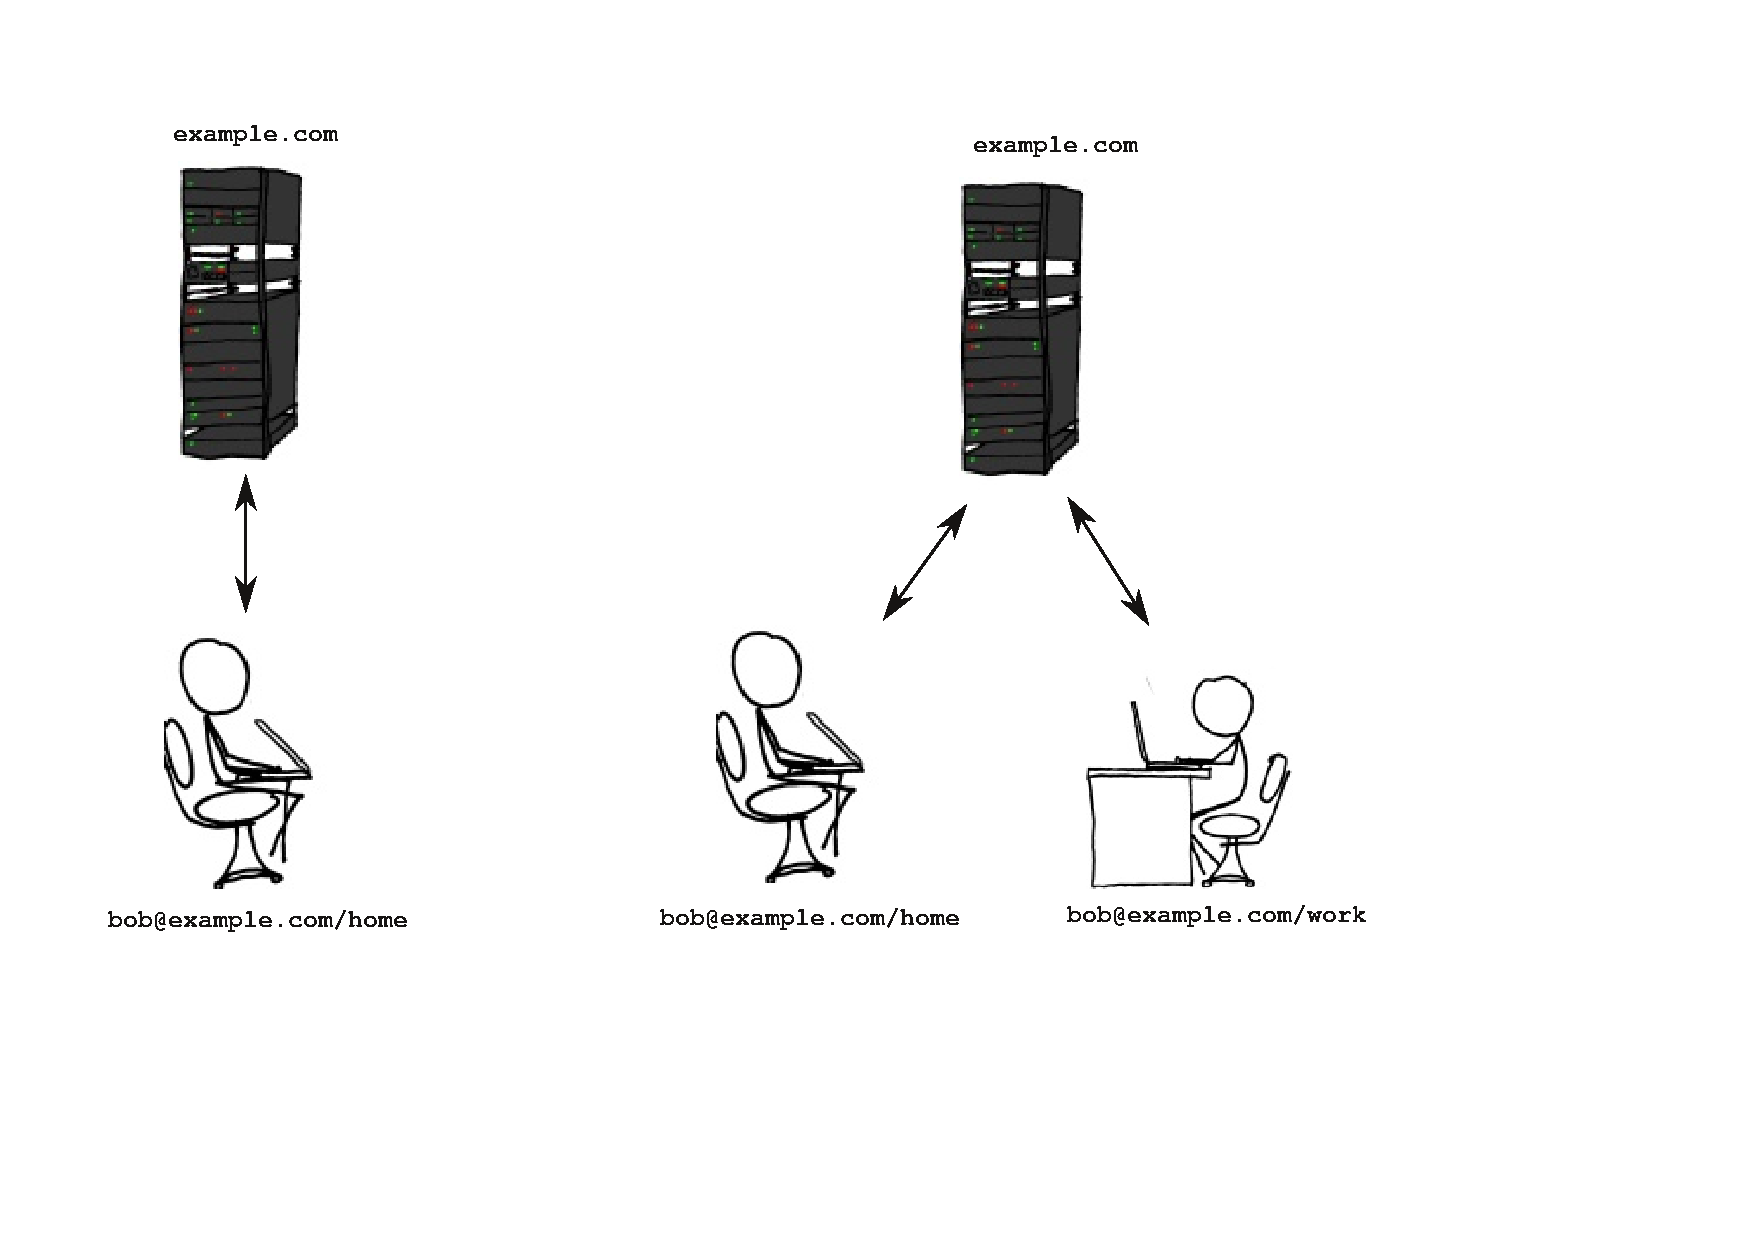
\includegraphics[scale=0.4]{../img/multiple-clients.pdf}
	\end{frame}
	
	\begin{frame}
		\frametitle{Incomplete conversations}
		\begin{block}{Problem:}
		Leads to incomplete conversations\\
		\end{block}
	\end{frame}
	
	\begin{frame}
		\frametitle{Single client}
		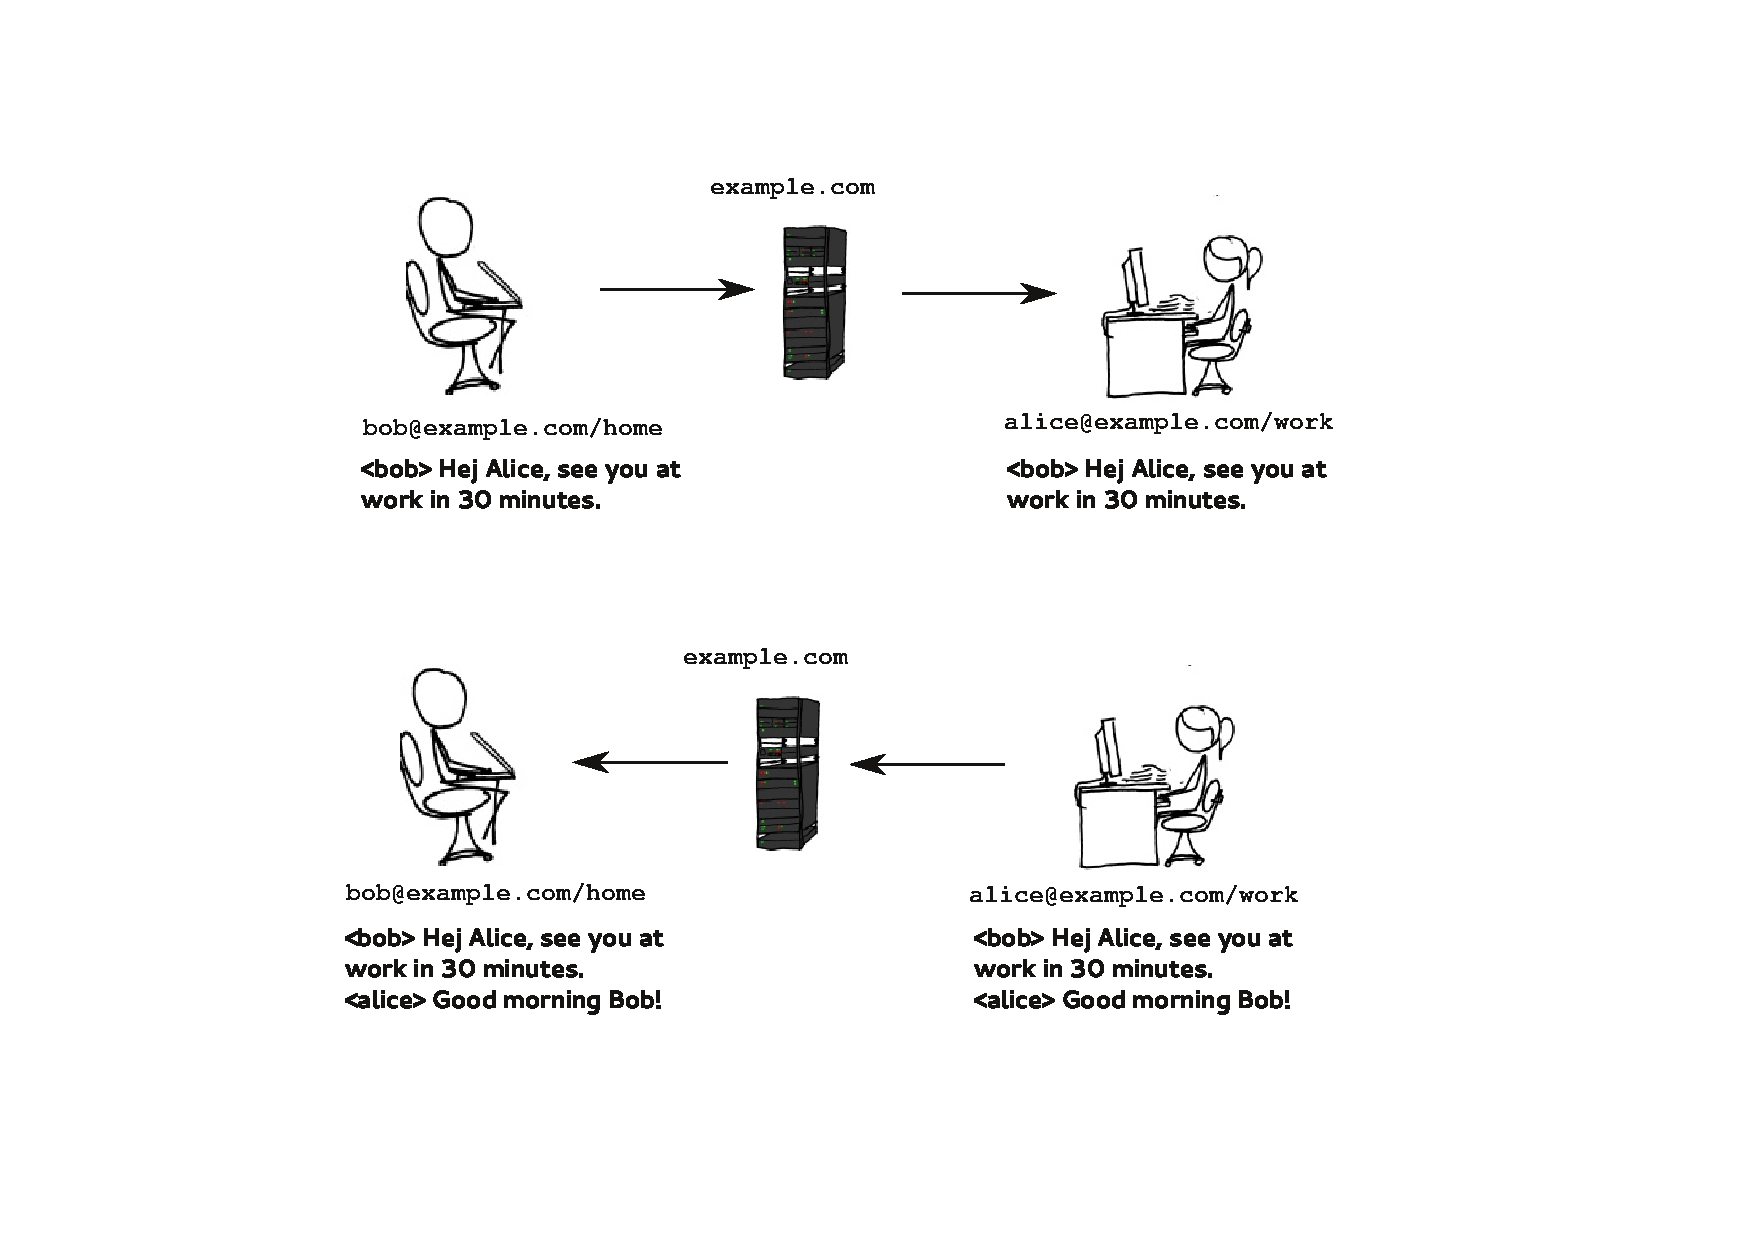
\includegraphics[scale=0.4]{../img/conversation1.pdf}
	\end{frame}
	
	\begin{frame}
		\frametitle{Two clients}
		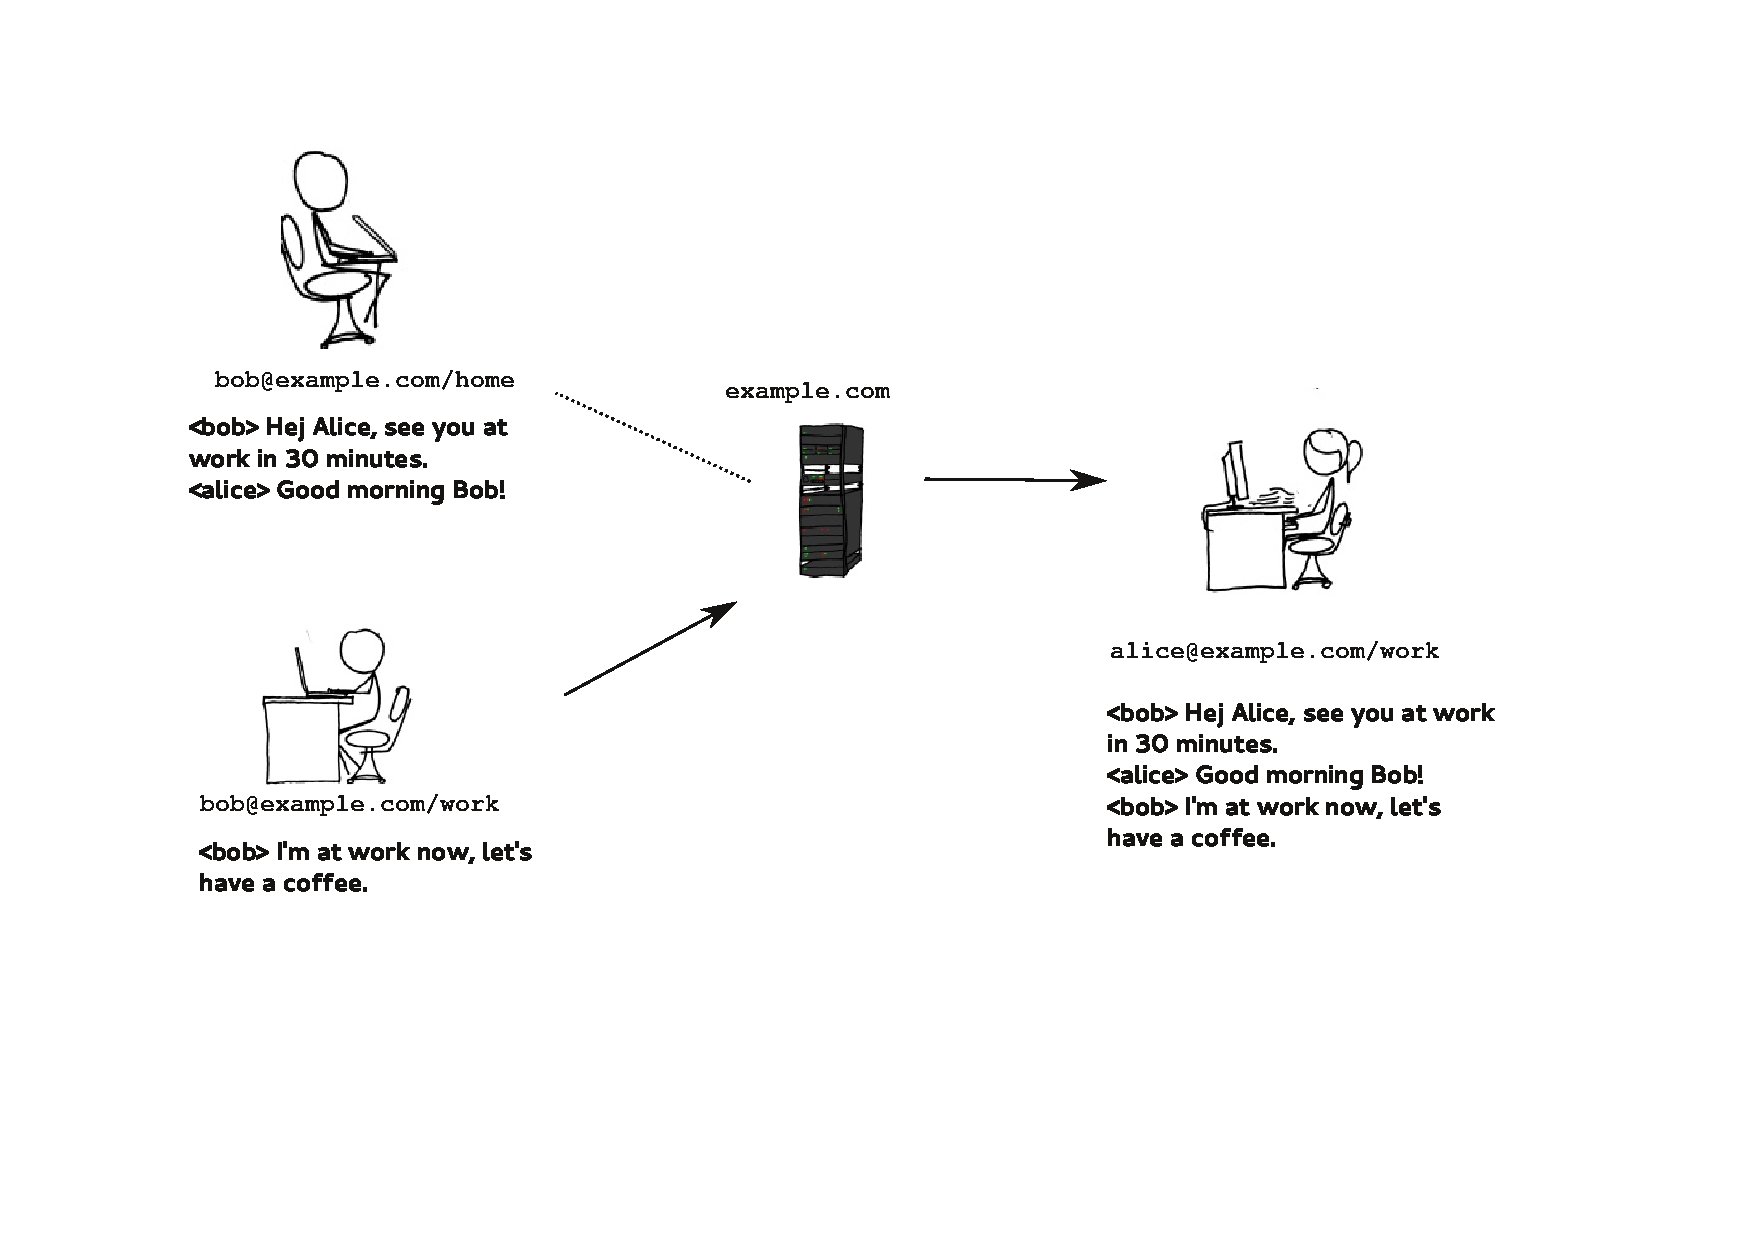
\includegraphics[scale=0.4]{../img/conversation2.pdf}
	\end{frame}
	
	\begin{frame}
		\frametitle{Two clients}
		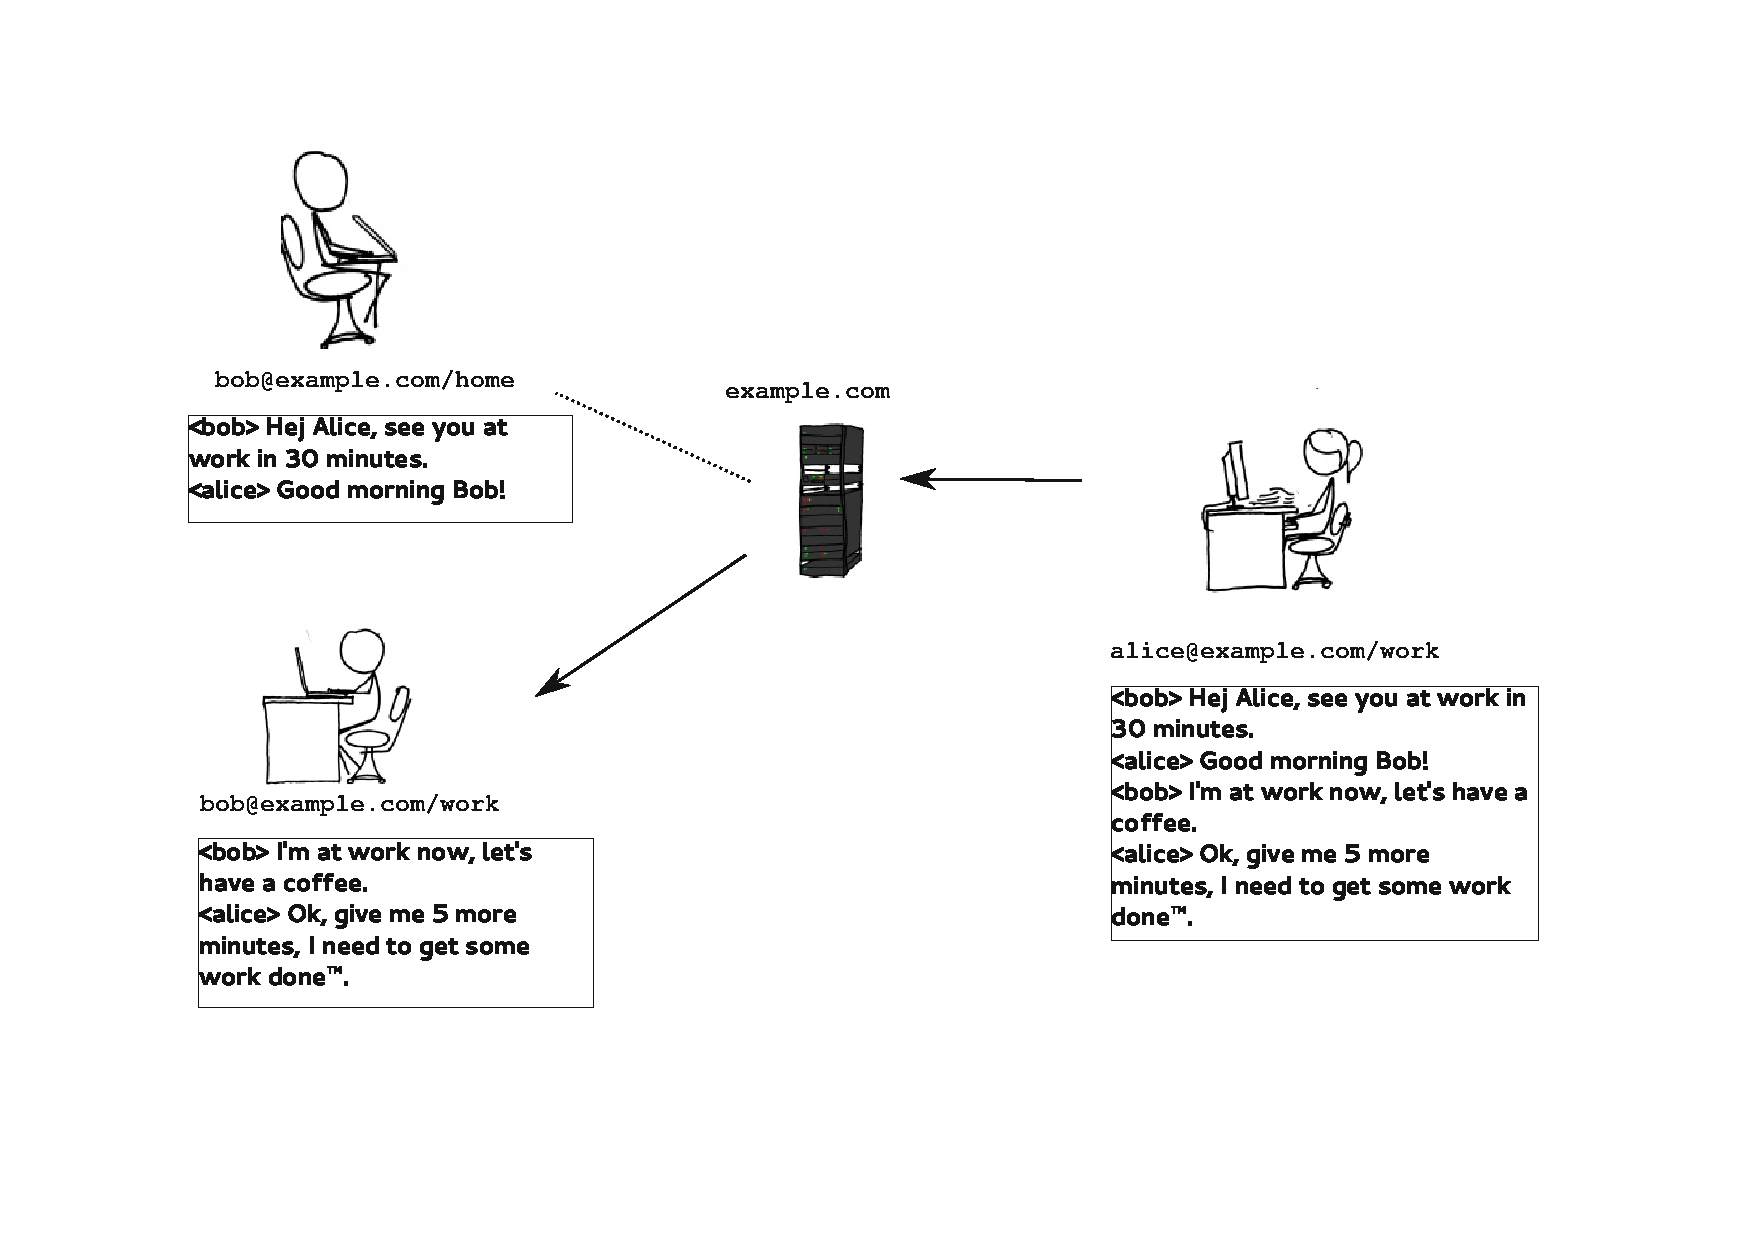
\includegraphics[scale=0.4]{../img/conversation3.pdf}
	\end{frame}
	
	\section{xmpproxy}
	\subsection*{}
	\begin{frame}
		\frametitle{Requirements}
		\begin{block}{Requirements}
			\begin{itemize}
					\item Every client has to see all incoming messages
					\item Outgoing messages have to be mirrored to other clients
			\end{itemize}
		\end{block}
		$\Rightarrow$ Put a proxy server inbetween actual client and server
	\end{frame}
	
	\begin{frame}
		\frametitle{One client, incoming and outgoing}
		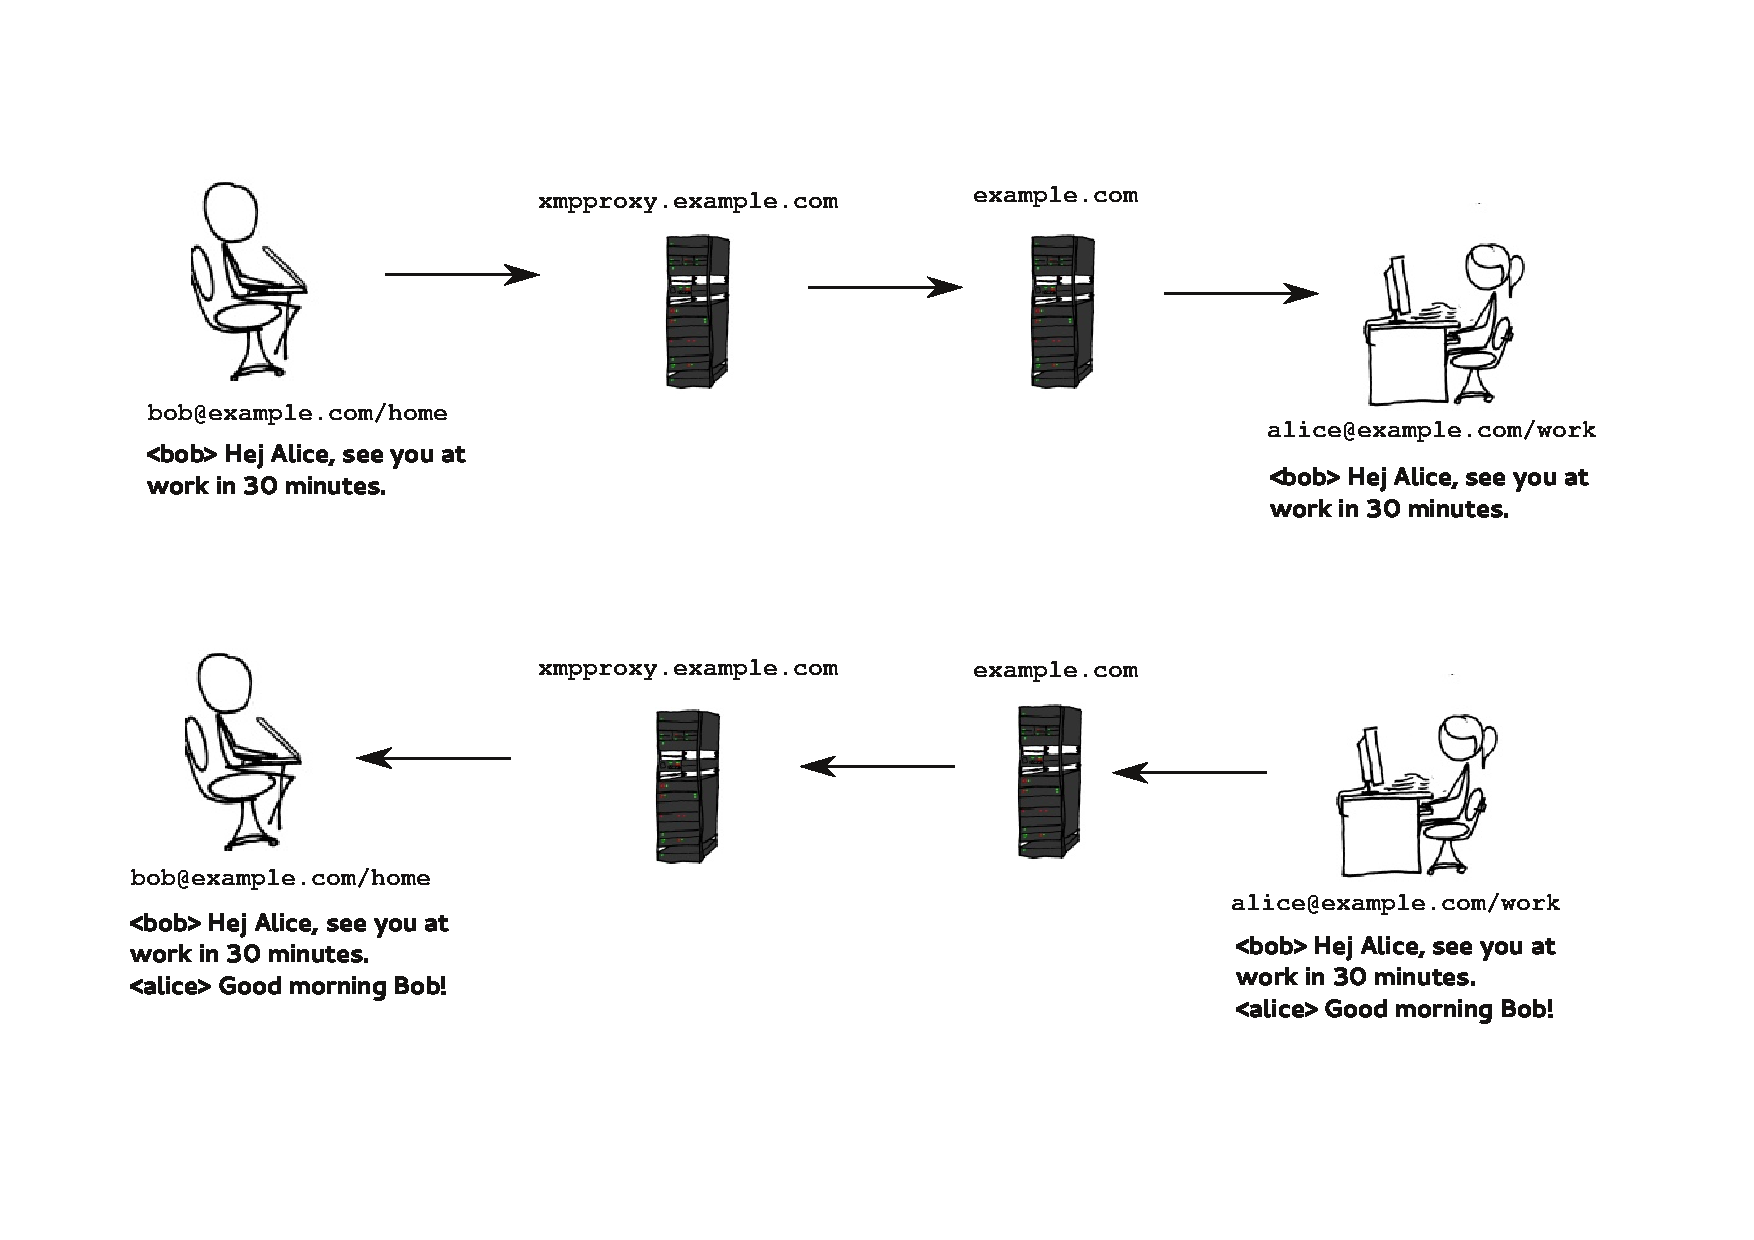
\includegraphics[scale=0.4]{../img/proxy1.pdf}
	\end{frame}
	
	\begin{frame}
		\frametitle{Two clients, outgoing}
		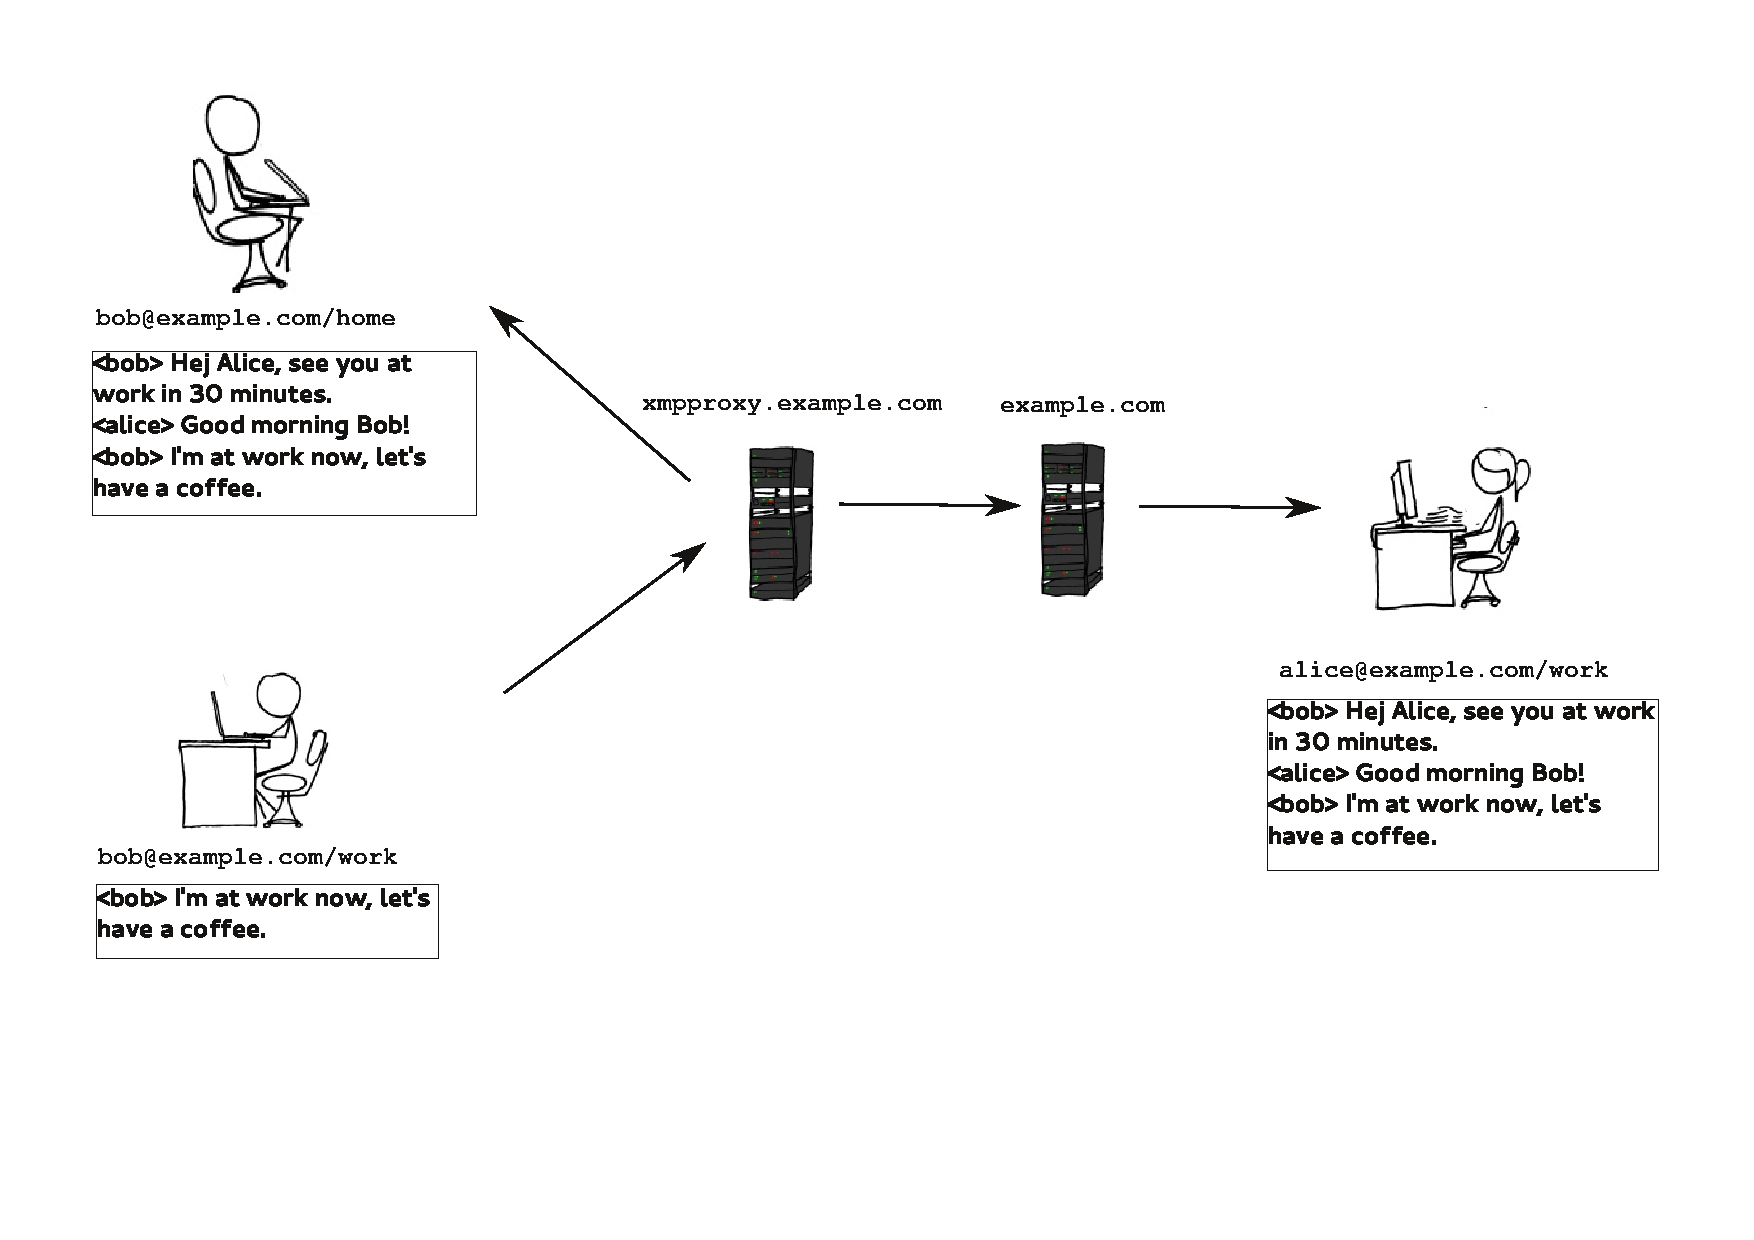
\includegraphics[scale=0.4]{../img/proxy2.pdf}
	\end{frame}
	
	\begin{frame}
		\frametitle{Two clients, incoming}
		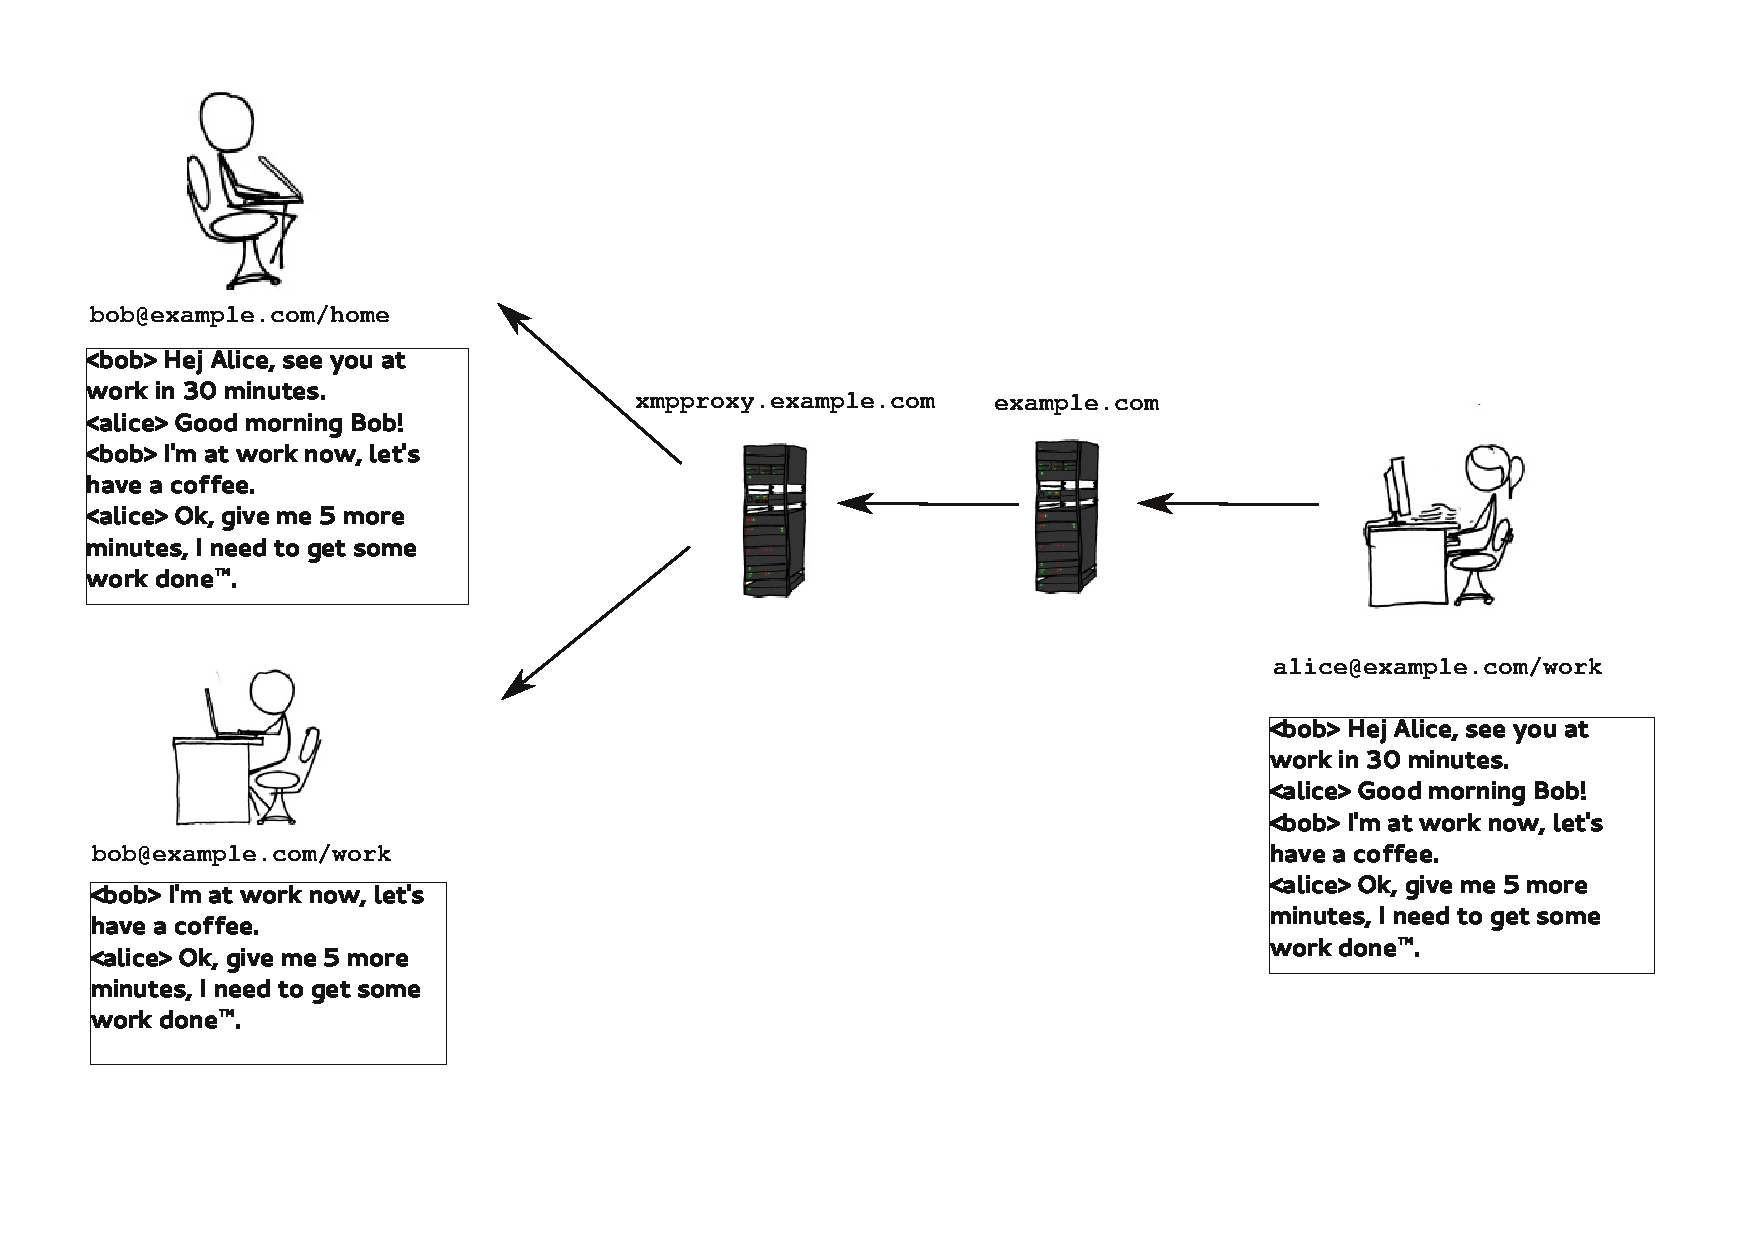
\includegraphics[scale=0.4]{../img/proxy3.pdf}
	\end{frame}

	\begin{frame}
		\frametitle{Usage}
		\begin{itemize}
			\item Connect to xmpproxy instead of actual jabber server
			\item Manage proxy accounts via \textit{root} bot in ``buddylist''

		\end{itemize}
	\end{frame}
\end{document}

